\documentclass[a4paper,12pt]{article}
\usepackage[utf8]{inputenc}
\usepackage[spanish]{babel}
\usepackage{color}
\usepackage{parskip}
\usepackage{graphicx}
\usepackage{multirow}
\usepackage{listings}
\usepackage{vmargin}
\usepackage{datetime}
\newdate{date}{19}{10}{2017}
\graphicspath{ {imagenes/} }
\definecolor{mygreen}{rgb}{0,0.6,0}
\definecolor{lbcolor}{rgb}{0.9,0.9,0.9}
\usepackage{epstopdf}
\usepackage{float}


\setpapersize{A4}
\setmargins{2.5cm}       % margen izquierdo
{1.5cm}                        % margen superior
{16.5cm}                      % anchura del texto
{23.42cm}                    % altura del texto
{10pt}                           % altura de los encabezados
{1cm}                           % espacio entre el texto y los encabezados
{0pt}                             % altura del pie de página
{2cm}     

\lstset{
    tabsize=4,    
%   rulecolor=,
    language=[GNU]C++,
        basicstyle=\tiny,
        aboveskip={1.5\baselineskip},
        columns=fixed,
        showstringspaces=false,
        extendedchars=false,
        breaklines=true,
        prebreak = \raisebox{0ex}[0ex][0ex]{\ensuremath{\hookleftarrow}},
        frame=single,
        showtabs=false,
        showspaces=false,
        showstringspaces=false,
        identifierstyle=\ttfamily,
        keywordstyle=\color[rgb]{0,0,1},
        commentstyle=\color[rgb]{0.026,0.112,0.095},
        stringstyle=\color{red},
        numberstyle=\color[rgb]{0.205, 0.142, 0.73},
%        \lstdefinestyle{C++}{language=C++,style=numbers}’.
}


\begin{document}
\title{Tarea de Laboratorio 3}
\author{
Christofer Fabián Chávez Carazas \\
\small{Universidad Nacional de San Agustín de Arequipa} \\
\small{Escuela Profesional de Ciencia de la Computación} \\
\small{Compiladores}
}
\date{\displaydate{date}}

\maketitle

\begin{large}
 \textbf{Problema}
\end{large}


\textbf{Realizar un programa que convierta una expresión regular a un autómata}

El programa está estructurado de la siguiente manera:

\begin{itemize}
 \item \textbf{format.h:} Archivo con la función que da formato a la expresión regular.
 \item \textbf{postfix.h:} Archivo con la función que transforma una expresión regular en su forma postfija.
 \item \textbf{automata.h:} Archivo con la estructura utilizada para guardar un autómata.
 \item \textbf{compilador.h:} Archivo con el compilador que convierte una expresión regular a un autómata.
 \item \textbf{main.h:} Archivo que corre el compilador.
 \item \textbf{utils.h:} Archivo con funciones adicionales.
 \item \textbf{error.h:} Archivo para el manejo de errores.
\end{itemize}

\begin{enumerate}
 \item \textbf{format.h}
 
 En mi programa el único cambio que se hace en la expresión regular es la inserción del ``.'' como operador de concatenación. El operador OR no cambia.


 \item \textbf{postfix.h}
 
 El algoritmo convierte la expresión regular en su forma postfija.
 


 \item \textbf{automata.h}

 Clase Autómata que guarda todos los datos como estados, entradas y transiciones. LA clase tiene un constructor, que recibe
 una entrada y el contador de estados, y genera el autómata para esa entrada. Contiene también una función
 que imprime el autómata en el formato dado en clases.
 



 \item \textbf{compilador.h}
 
 Contiene la función \textit{run} que llama a la función para formatear y a la función para convertir a la forma postfija.
 Luego, evalúa la expresión. Al final imprime el autómata resultante. También tiene una función para cada operación.
 

 \item \textbf{main.cpp}
 
 El main crea una instancia del compilador y lo ejecuta con la expresión regular leída.
 

 
 \item \textbf{utils.h}

 Funciones usadas en otros archivos.
 

 \item \textbf{error.h}
 
 Archivo con los tipos de errores y una función para el manejo de errores.
 

\end{enumerate}

\begin{large}
 \textbf{Experimentos y Resultados}
\end{large}

 Para imprimir el caracter nulo o vacío se utiliza la colita de chancho.

\begin{itemize}
 \item $(b|(b^{*}a)^{*})a$
 \begin{figure}[H]
  \centering
  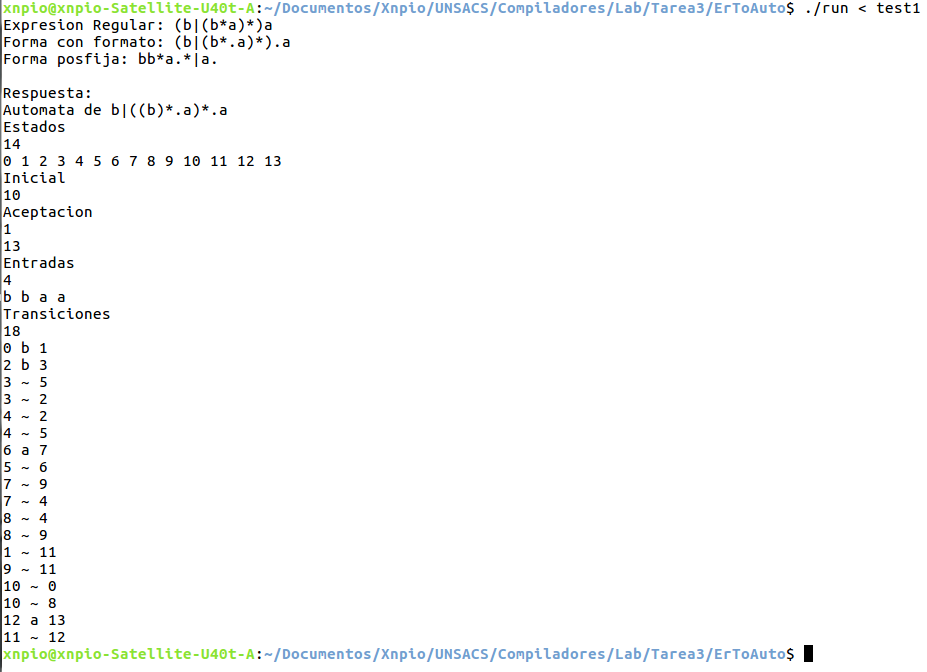
\includegraphics[scale = 0.4]{1.png}
 \end{figure}
 \item $(abc)^{*}$
 \begin{figure}[H]
  \centering
  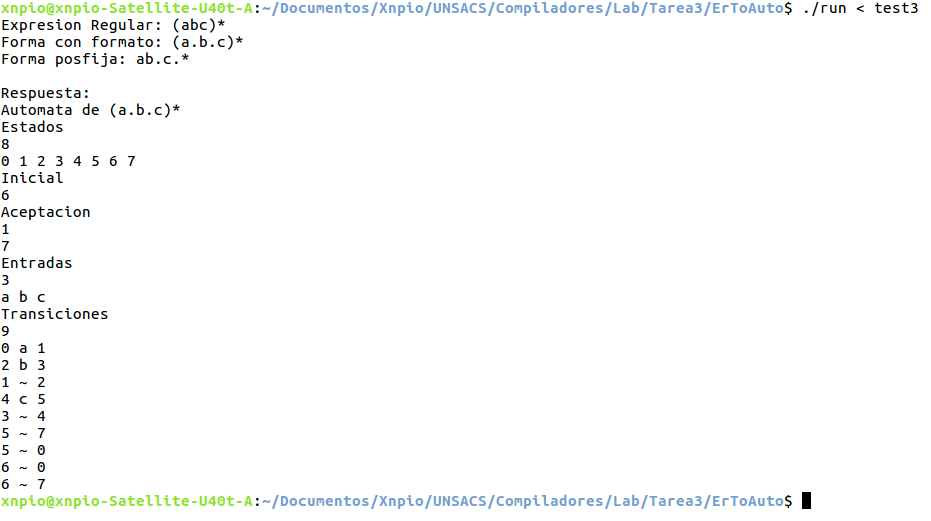
\includegraphics[scale = 0.4]{2.png}
 \end{figure}
 \item $(b|bc)^{+}$
 \begin{figure}[H]
  \centering
  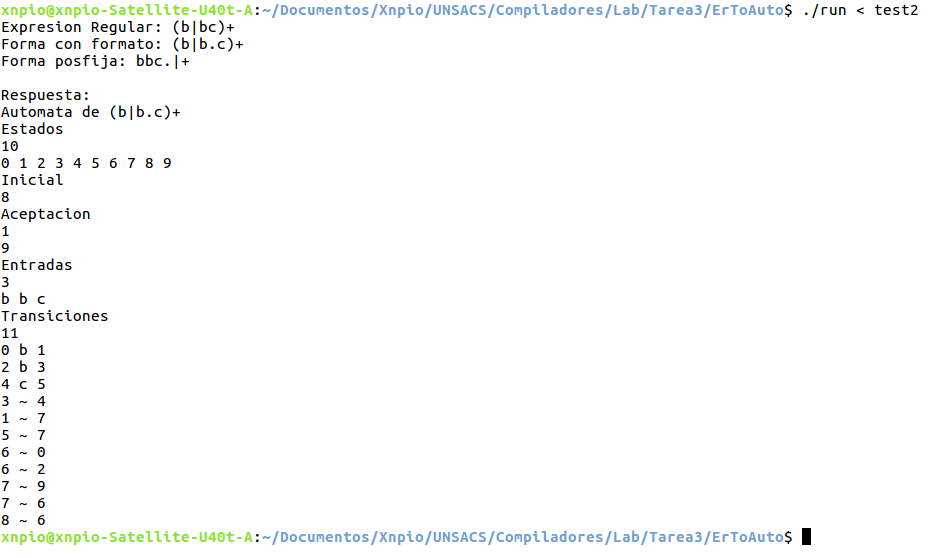
\includegraphics[scale = 0.4]{3.png}
 \end{figure}
 \item $(a^{*}|b^{+})^{+}$
 \begin{figure}[H]
  \centering
  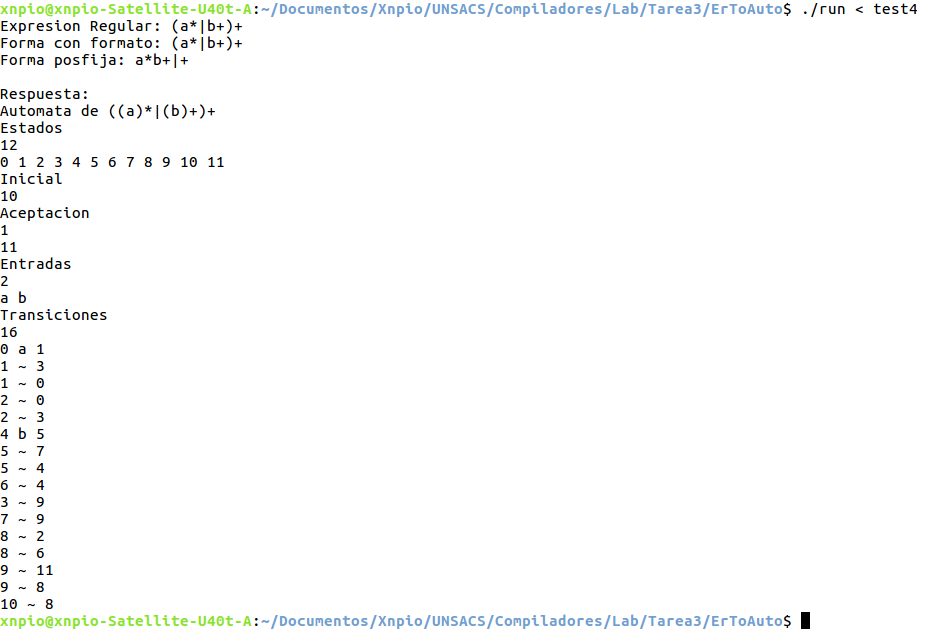
\includegraphics[scale = 0.4]{4.png}
 \end{figure}



 
\end{itemize}




\end{document}

